\[
    \begin{gathered}
        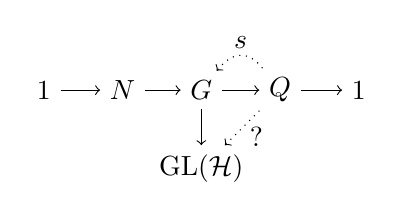
\begin{tikzpicture}
            \node (A) at (-2, 0) {$1$};
            \node (B) at (-1, 0) {$N$};
            \draw[->] (A) -- (B);
            \node (C) at (0, 0) {$G$};
            \draw[->] (B) -- (C);
            \node (D) at (1, 0) {$Q$};
            \node (E) at (2, 0) {$1$};
            \draw[->, dotted]  (D) .. controls (0.6, 0.5) and (0.4, 0.5) .. (C) ;
            \node at (0.5, 0.6) {$s$};
            \draw[->] (C) -- (D);
            \draw[->] (D) -- (E);
            \node (F) at (0, -1) {$\mathrm{GL}(\mathcal{H})$};
            \draw[->] (C) -- (F);
            \draw[<-, dotted] (F) -- (D);
            \node at (0.7, -0.6) {?};
       \end{tikzpicture}
    \end{gathered}
\]